In general the \textbf{control theory} deals with the formulation of a \textbf{control law} $u(t)$ above a given physical system with a given dynamics. The system $C$, the so called \textbf{Controller}, should be applied on the real plant such that $y = r$ for a set of signals of interest. The command $u(t)$ is defined into the system $C$ in a proper way.\\

\begin{figure}[h]
    \centering
    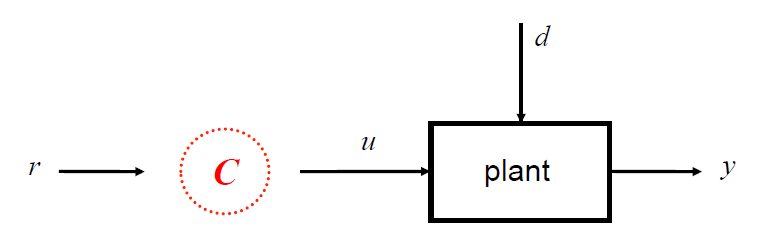
\includegraphics[scale=0.8]{NonLinearControl/images/ControlScheme.png}
    \caption{Classical structure of a controlled plant}
    \label{fig:enter-label}
\end{figure}

\noindent
In this field topics of interest are: (a) The nonlinear stabilization of the real  plant, (b) the nonlinear Tracking, (c) The specification of Desired Behaviour of the System. 

\section{Non linear Stabilization and Tracking}
In the case that the \textbf{tasks of a Control System} involve large range or high speed motions, non linear behaviours and effects can be a problem, for this reason \textbf{non linear control} is necessary to achieve some objectives. \\
Generally speaking, the tasks of a control system can be divided into two categories: 
\begin{itemize}
    \item \textbf{Stabilization} (or Regulation), here a control system called a \textit{stabilizer} (or regulator), is designed so that the \textbf{closed-loop} system is stable around an equilibrium point (examples: temperature regulation, altitude control...);
    \item \textbf{Tracking} (or Servo), here the design objective is to build a controller, called the \textit{tracker}, which has the task to ensure that the system could track a desired \textbf{time-varying trajectory} (examples: making a robot hand draw straight lines or circles, making an aircraft fly along a specified path...)
\end{itemize}

\section{Specifying the desired behaviour}
In linear control, the desired behaviour of a control system can be specified either in the time-domain by providing specifications like rise time, overshoot and settling time) or  in the frequency domain in terms of regions in which the \textit{loop transfer function} (usually indicated with $L(s)$) should lie at high and low frequencies.\\
However, \textbf{systematic specifications} for nonlinear systems (except those equivalent to linear system) are not obvious: at first a frequency-domain specification is not available, the response of the system to one command does not reflect its response to another command. As a result, for nonlinear system, one often try to find some \textbf{qualitative} specifications in the operating region of interest. Some common characteristics are: Stability (guaranteed for the nominal model), Robustness, Cost, Accuracy and speed of response.

\section{A general procedure for Control Design}
Given a physical system to be controlled, one typically goes through the following standard procedure:
\begin{enumerate}
    \item specify the desired behaviour, and select the actuators and sensors; 
    \item model the physical plant by a set of differential equations; 
    \item design a control law for the system;
    \item analyze and simulate the resulting control system;
    \item implement the control system in hardware;
\end{enumerate}

\section{Available methods for nonlinear controllers}
As in the analysis, we have not a general method to \textbf{design a nonlinear controller}, even in this case we have a collection of techniques which are either alternative or complementary and each applicable to a class of nonlinear control problems.\\
\subsection{Trial and error}
It is based on the analysis method provided before, like the \textit{phase plane method} and the \textit{Lyapunov analysis}. The design strategy deploys this technique in a way similar to the loop-shaping. This technique may work sometimes but in complicated situation it fails.

\subsection{Feedback linearization}
As discussed in the previous paragraphs, one of the main steps for design a controller (the first in particular) is to derive a meaningful model for the plant. \textbf{Feedback linearization} deals with techniques for \textit{transforming the original system models into equivalent models of a different simpler form}. Can be used in a proper way as a strategy for design nonlinear controller. The \textbf{basic idea} is to linearize (fully or in part) the nonlinear plant and  then apply the well-known techinques to complete the control design.\\
It is  appliable to a number of practical cases. As a \textit{drawback} it does not guarantee robustness against \textbf{disturbances} and \textbf{parameters uncertainty}.
\subsection{Robust control}
In the great majority of the control techniques the controller is designed according to the \textbf{nominal model of the plant/physical system}. In pure \textbf{model-based} design strategies uncertainties are neglected. In \textbf{robust nonlinear control} (eg. \textit{Sliding Mode Control}), on the other hand, the controller is designed by exploiting both nominal plant and some characterization of the model uncertainties.\\


\subsection{Adaptive control}
\textbf{Adaptive control} is a technique to deal with \textbf{uncertain or time-varying systems}. Despite these alternatives, nowadays, adaptive control techinques are used when one have to face with system with \textit{known dynamic structure} but \textbf{unknown constant or time-varying parameters}. \\
There are quite strong results for linear systems concerning this strategy, but  also for nonlinear systems with \textbf{measurable state} and \textbf{linearly parametrizable dynamics} have been deployed some methods. When it is possible to design such type of controller it represents an alternative or a complementary part for the robust control design. 

\subsection{Gain scheduling}
\textbf{Gain scheduling} is a method which make a try to apply well-known linear techniques to control nonlinear systems. It was developed for the trajectory control of aircraft. \\
The \textbf{idea behind} this technique is to collect a \textbf{set of operating points} which may cover the range of the system operation. Then, at \textbf{each of these points}, the designer makes a linear time variant approximation to the plant dynamics and build a \textbf{linear controller} for each linearized plant. What happen between two operating points? The parameters are interpolated, or \textbf{scheduled}, providing a global compensator. Maybe Gain Scheduling is the simplest method for designing nonlinear controllers, but the main problem is that one have only limited guarantees in stability in non linear operations; another drawback is the necessity of computing a cospicuous number of linear controllers.
